%--------------------------------------------------------------------------------
%----------------------------------------------------------------------
\section{Validation}\label{sec:validation}
Unit tests have been written with the JUnit library that validate the classes the user works with the most: \lstinline{Node}, \lstinline{Relation}, \lstinline{NodeList}, \lstinline{RelationList}, \lstinline{FxWrapper}, \lstinline{FxWrapper}'s subclasses, \lstinline{Placement} and \lstinline{Placement}'s subclasses. The unit tests include the various ways of instantiating new objects, calling their methods with extreme values and in the case of the \lstinline{Placement} tests, they verify the calculations made to place a node in a certain respect to another node. These tests all worked as expected.
\par Due to the visual nature of GreenMirror, further verification is based on an extensive system test, written for use with the Groovy script model initializer. This test also works to some extent as a unit test: it tests several classes and specific functionalities. Furthermore, it showcases and explains how certain functionalities work and how they can be used. Among other sub-tests, it tests the following:
\begin{itemize}
\item setting the duration of animations;
\item using parameters from state-transition names;
\item adding nodes;
\item setting the FX of nodes;
\item altering the general properties of nodes;
\item altering properties specific for shape nodes (rectangle, circle and text nodes);
\item altering properties of a rectangle node;
\item altering properties of an image node;
\item altering properties of a text node;
\item adding and removing simple relations between nodes;
\item adding and replacing placement relations;
\item using rigid placement relations;
\item using chained, rigid placement relations; and
\item removing nodes.
\end{itemize}
\par A coverage of 84.8\% has been achieved with all tests combined. GreenMirror uses the \lstinline{@NonNull} annotation with fields and method arguments and return types. Not all sub-packages of Java formally guarantee that they return a non-null object (although they do informally), resulting in several non-null checks that are effectively futile and practically non-reachable code.
\par All test cases discussed in \cref{sec:intro;sub:project} have been successfully visualized. A screenshot of the results are illustrated in \cref{fig:greenmirror_ferryman,fig:connectfour,fig:phil}. They were all fairly easy to construct using the Groovy script model initializer. The realization of the ferryman case was a bit more elaborate compared to the realization discussed in \cref{sec:ferryman}, although the case itself and \cref{fig:greenmirror_ferryman} are essentially the same for both realizations. The test case, for example, also includes the state-transition where one cargo object 'eats' another. \Cref{tab:testcases} lists all relevant results of the three test cases.
\newpage\begin{longtable}{|l|r|r|r|p{6.7cm}|}
\caption{test case results}\label{tab:testcases}\\
\hline \textbf{Test case} 
     & \multicolumn{1}{|p{0.9cm}|}{\textbf{lines of code}}
     & \multicolumn{1}{|p{1.0cm}|}{\textbf{trace length}} 
     & \multicolumn{1}{|p{1.2cm}|}{\textbf{init. time}\footnote{Initialization time: the time GreenMirror needs to interpret the model and generate the visualizations.}} 
     & \textbf{notable visualizations and used functionalities} \\
\hline Ferryman            & 109 & 20 & $\approx$ 48 s & Parametrized state-transition names, rectangle FX types, image FX types, node resizing, node rotation, node removal, placement relations, rigid placement relations, non-placement relations, relation replacements, colour gradients \\
\hline ConnectFour         &  91 & 10 &  $\approx$~~8 s & Parametrized state-transition names, rectangle FX types, circle FX types, text FX types, node grid generated with \texttt{GridBuilder,} node creation during state-transition, colour gradients, font size setting, placement relations, relation replacements, complex model logic (determining the cell number from the column number), model failing (if an invalid move is encountered on the trace), altering animation duration \\
\hline Dining Philosophers & 132 & 15 & $\approx$ 10 s & Parametrized state-transition names, circle FX types, image FX types, image alteration during state-transition, node rotation, placement relations, non-placement relations, relation replacement, model failing (if an impossible state-transition is encountered) \\
\hline\end{longtable}
\begin{figure}[h]
\centering
    \begin{subfigure}[b]{0.53\textwidth}
    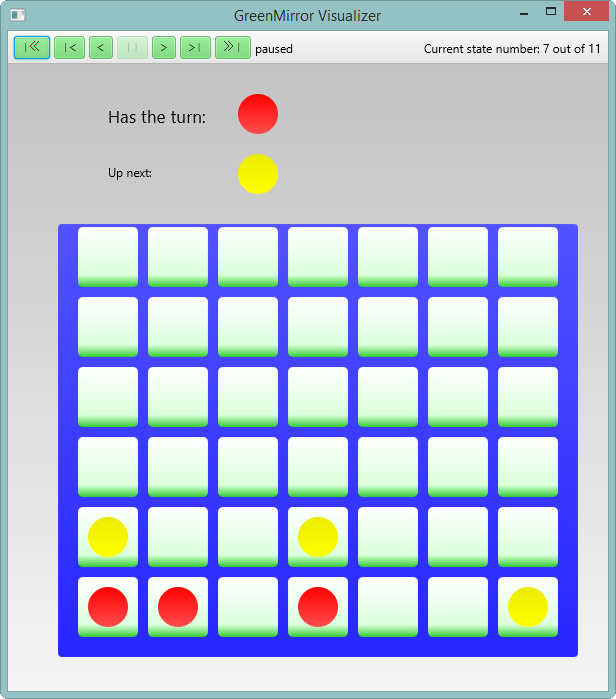
\includegraphics[width=\textwidth]{images/connectfour}
    \caption{ConnectFour}\label{fig:connectfour}
    \end{subfigure}
    ~
    \begin{subfigure}[b]{0.44\textwidth}
    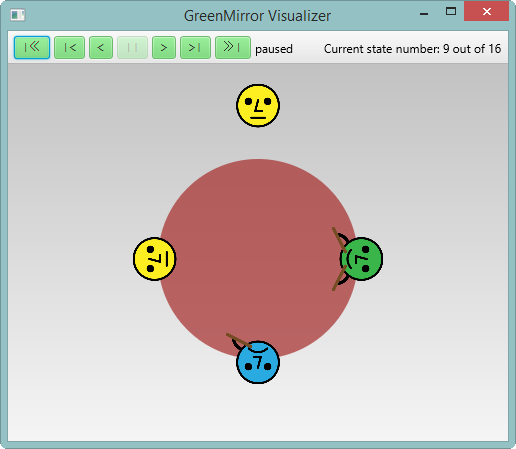
\includegraphics[width=\textwidth]{images/phil}
    \caption{Dining Philosophers}\label{fig:phil}
    \end{subfigure}
\caption{screenshots of two of the test cases}\label{fig:connectfour_phil}
\end{figure}
\par The following list discusses how each requirement and use case is implemented and validated, in the same order as they were defined in \cref{sec:intro;sub:project}.
\begin{description}
\item\textbf{\Cref{req:extensible,uc:extend}}\\The framework is easily extensible due to the use of interfaces and abstract classes. One example is the \lstinline{FxWrapper} class: support for new FX elements can be easily added by extending \lstinline{FxWrapper}. Also, the use of common design patterns makes extension more easy. See \cref{app:ext} for a full list of extensible parts.
\item\textbf{\Cref{req:maintainable}}\\The use of common design patterns, extensive documentation and the use of the checkstyle plugin of Eclipse are the primary means of making the framework maintainable. Especially the model-view-controller pattern is important because it tells which classes are responsible for what. More details on the design patterns can be found in \cref{sec:design;sub:patterns}.
\item\textbf{\Cref{req:aware_model,uc:model_aware,uc:model_source}}\\The application becomes aware of the user's model via the use of the model initializers: implementations of \lstinline{ModelInitializer}. It depends on the implementation how this is done. The choice of the implementation is how \cref{uc:model_aware} is supported: by use of the command line options and specifically the \lstinline{ModelCommandLineOptionHandler} class that handles the choice. This option handler accepts one argument: the source of the model (\cref{uc:model_source}) and it depends on the \lstinline{ModelInitializer} implementation how this source is given (for example: a file name or a model name).
\item\textbf{\Cref{req:aware_trace,uc:trace_source}}\\The user can pass his choice for the trace source via the command line and gets handled by the \lstinline{TraceCommandLineOptionHandler} class. The user's chosen \lstinline{TraceSelector} implementation then retrieves the trace and that is how the application becomes aware of the trace.
\item\textbf{\Cref{req:show_vis,req:show_vis_geom,req:show_vis_text,req:show_vis_imag,req:show_vis_anim,req:show_vis_plac,uc:vis}}\\A few examples of where the validation of these requirements is visible (as seen in \cref{fig:greenmirror_ferryman,fig:connectfour,fig:phil}): the ConnectFour test case visualizes rectangles, circles (\cref{req:show_vis_geom}) and text (\cref{req:show_vis_text}); the ferryman test case visualizes images (\cref{req:show_vis_imag}); and the dining philosophers test case visualizes the placement of nodes with respect to other nodes (\cref{req:show_vis_plac}). All test cases visualize simple animations (\cref{req:show_vis_anim}), which of course is not visible in the figures. The fact that these test cases can be visualized validates \cref{req:show_vis,uc:vis}.
\item\textbf{\Cref{req:log,uc:log}}\\This is implemented by the \lstinline{Log} class, as is discussed in \cref{sec:features;sub:log} and visible in \cref{fig:log} (page~\pageref{fig:log}).
\item\textbf{\Cref{req:browse,uc:browse}}\\Browsing from state to state is implemented by use of a toolbar with navigation buttons. The workings of these buttons are handled by the \lstinline{Visualizer} controller in cooperation with the \lstinline{PlaybackState} implementations and \lstinline{ToolbarButton} class. \Cref{sec:design;sub:patterns} discusses the playback state and its effect on the toolbar buttons. The buttons are also visible on any of the screenshots of GreenMirror in this report.
\item\textbf{\Cref{req:nodelay,req:nocrash}} \\Smoothly transitioning from state to state (\cref{req:nodelay}) is implemented by cleaning up resources every time the visualizer is closed. This 'resets' the server so a new client can connect. Crashing is prevented (\cref{req:nocrash}) by properly catching exceptions while the model is being loaded: this makes sure the visualizer will not crash during the state-transitions. If any exceptions are thrown, they will be displayed in the log.
\end{description}